\documentclass{beamer}

%Para simbolo independencia
\newcommand\independent{\protect\mathpalette{\protect\independenT}{\perp}} 
\def\independenT#1#2{\mathrel{\rlap{$#1#2$}\mkern2mu{#1#2}}} 



\mode<presentation>
{
  \usetheme{Copenhagen}
  \useoutertheme{infolines}    
  \usecolortheme{default} 
  \usefonttheme{default}  
  \useinnertheme{circles}  
  \setbeamertemplate{navigation symbols}{}
  \setbeamertemplate{caption}[numbered]  
} 

\usepackage{booktabs}
\usepackage{dcolumn}

\usepackage[english]{babel}
\usepackage[utf8x]{inputenc}
\usepackage{pgfpages}
\usepackage{amsmath}
\usepackage{amssymb}
\usepackage{ragged2e}
\usepackage{color} %color
\usepackage{url} %link a web
\usepackage{xcolor} % Permite definir colores.
\definecolor{forestgreen}{RGB}{34,139,34}
\pgfpagesuselayout{resize to}[
  physical paper width=8in, physical paper height=6in]

%Paquetes para ecuaciones con cajas de color
\usepackage[skins,theorems]{tcolorbox}
\tcbset{highlight math style={enhanced,
		colframe=red,colback=white,arc=0pt,boxrule=1pt}}
% Frame 1
\title [] {Exposure to information about economic inequality, opportunity beliefs and redistributive preferences: Results of survey experiments among Chilean population}

\author[]
{L.~Maldonado\inst{1}\inst{3} \and J.C.~Castillo\inst{1}\inst{2} \and M.C.~Ayala\inst{1} \and J.~Atria\inst{1}\inst{2}} 

\institute[]
{
\inst{1}
Instituto de Sociología, Pontificia Universidad Católica de Chile
\and
\inst{2}
Centre for Social Conflict and Cohesion Studies (COES)
\and
\inst{3}
Research Center for Integrated Disaster Risk Management (CIGIDEN)
}


\date{19th November, 2018}

\begin{document}

\frame{\titlepage}
% Frame 2
\section[Contenidos]{} % [{} suprimen "contenidos" de tabla de contenidos
\frame{\tableofcontents}

% Intro
\section{Introduction}

\begin{frame} [allowframebreaks]
\frametitle{}

\begin{itemize}
\justifying	
\item \textbf{Objective}: We examine whether exposure to objective information about economic inequality affects beliefs about the opportunity structure in society and redistributive preferences. 
\medskip
\medskip
\item We collected convenience samples via advertisements on Facebook for pilot study. 
\medskip
\medskip
\item We plan to run our survey experiment via Survey Sampling International (SSI), an online panel company that produces samples which are typically more diverse than those collected through online convenience samples, such as Amazon's Mechanical Turk website (Berinsky et al. 2016).
\end{itemize}  

\end{frame}

% Literatura
\section{Patterns in Chilean population}

%Frame 19
\begin{frame}{Economic development and poverty in Chile} 
\begin{center}
	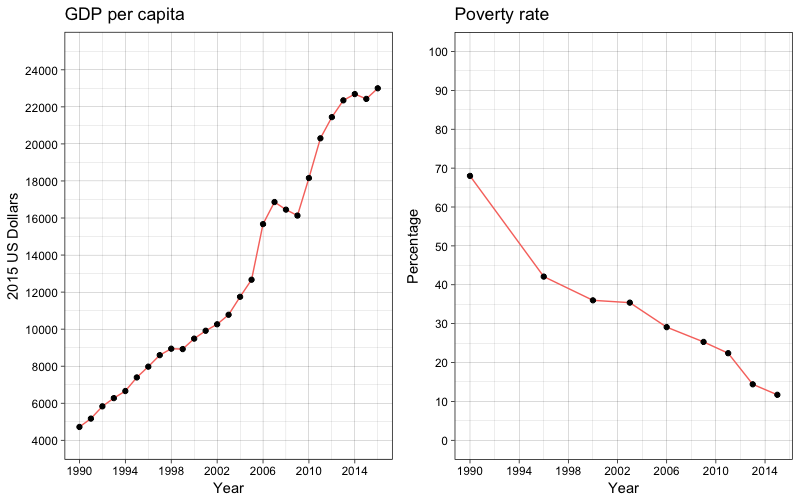
\includegraphics[height=6.5cm]{Rplot4.png}
\end{center}

{\footnotesize Source: OECD 2018 and PNUD 2017.}

\end{frame}


%Frame 19
\begin{frame}{Income inequality and social expenditures} 
\begin{center}
	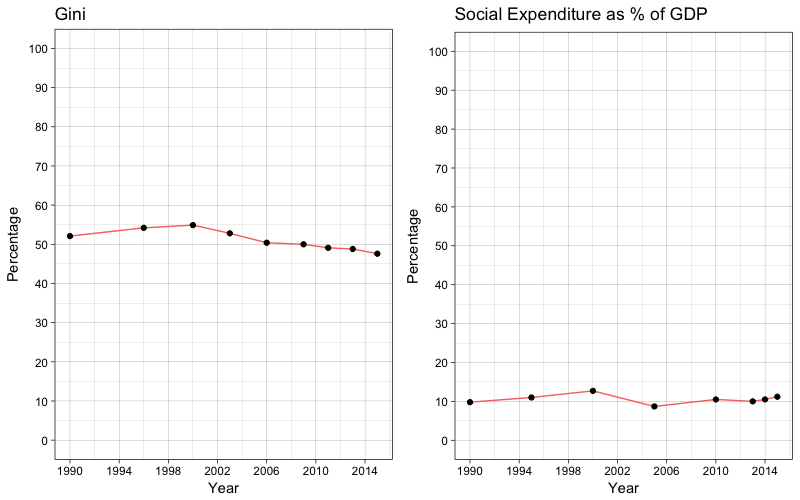
\includegraphics[height=6.5cm]{Rplot5.png}
\end{center}

{\footnotesize Source: OECD 2018 and PNUD 2017.}

\end{frame}


%Frame 19
\begin{frame}{Redistributive preferences} 
\begin{center}
	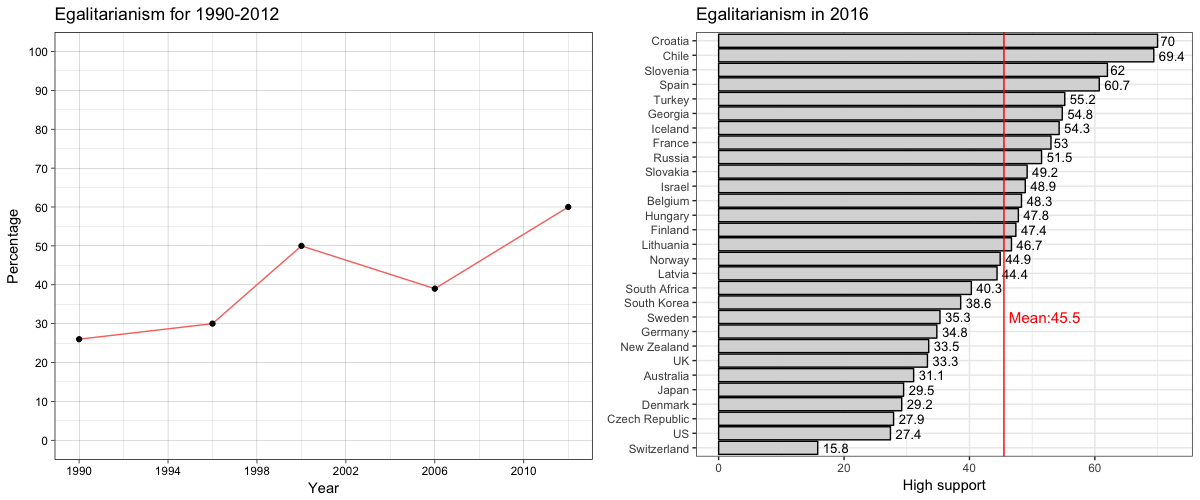
\includegraphics[height=5.0cm]{Rplot6.png}
\end{center}

{\footnotesize Source: WVS 1990-2012 and ISSP 2016. Figure on the left is level of agreement with \textit{Incomes should be made more equal}; Figure on the right is option \textit{Definitely should be the government's responsibility to reduce income differences between the rich and the poor}}

\end{frame}

%Frame 19
\begin{frame}{Perception of economic inequality} 
\begin{center}
	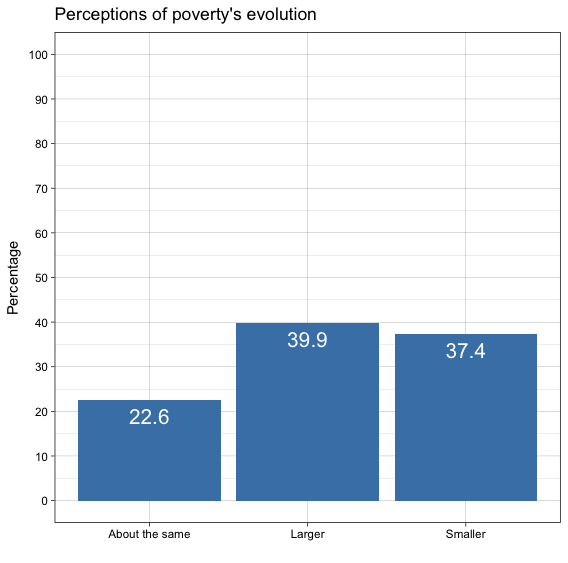
\includegraphics[height=5.8cm]{Rplot7.png}
\end{center}

{\footnotesize Source: Pilot study (non representative of Chilean population). Question is: \textit{Do you think that the quantity of poor people in Chile today is larger, smaller or about the same as it was 20 years ago?}}

\end{frame}






%Intro
\begin{frame}{Hypothesis} 

\begin{itemize}
\justifying	
\item \textbf{Expectations for USA}
\medskip
	\begin{enumerate}
	\justifying
	\item H1a: Perceptions of increasing economic inequality spark skepticism about the existence of economic opportunity. 
	\medskip
	\item H2a: Awareness of rising inequality triggers support for equity-enhancing policies (business and government).
	\medskip
	\item H3a: Opportunity beliefs mediate the effect of perceptions of increasing economic inequality.
	\end{enumerate}
\medskip
\medskip
\item \textbf{Expectations for Chile}
\medskip
	\begin{enumerate}
	\justifying
	\item H1b: Awareness of decreasing poverty increases support for individual factors.
	\medskip
	\item H2b: Awareness of decreasing poverty increases support for opportunity-enhancing policies (gratuidad and pension reform). 
	\medskip
	\item H3b: Opportunity beliefs mediate the effect of perceptions of increasing economic inequality.	
	\end{enumerate}
\end{itemize}


\end{frame}


% Methodology
\section{Research design}

\begin{frame}{Datos}

\begin{enumerate}
\justifying
\item Convenience sample collected via advertisements on Facebook for pilot study on 6th November 2018.
\medskip
		\begin{itemize}
		\justifying
		\item N= 502.
		\medskip
		\item Mean duration: 9,45 minutes.
		\medskip
		\item 24\% of participants do not finish the questionary. 68\% of them select correct answer in the attention check. Effective sample has 334 respondent. Attrition and ability to pass manipulation checks are not systematic across treatment conditions (chi-squared test, p-value $>$ 0.10).	
		\medskip
		\item Sociodemographic profile: 64\% women, averaged age is 45 years, 61\% of respondents has tertiary education, 51\% are workers.	
		\end{itemize}	
\medskip
\item Questionary and random assignment by using Qualtrics.			
\end{enumerate}

\end{frame}


% Slide
\begin{frame}{Treatments}

\begin{itemize}
\justifying
\item Three conditions
\medskip
	\begin{enumerate}
	\justifying
	\item \textbf{Poverty condition}: Information about evolution of poverty in Chile in period 1990-2015.
	\medskip
	\medskip
	\item \textbf{Control condition}: Information about consume of cigarette in Chile during the last decades.
	\medskip
	\medskip
	\item \textbf{Inequality condition}: Information about income inequality in Chile in terms of index 10/10 that shows Chile as one of the countries with the highest income inequality within OECD. 
	\end{enumerate}	
\end{itemize}	
	
\end{frame}	


%Frame 19
\begin{frame}{} 
\begin{center}
	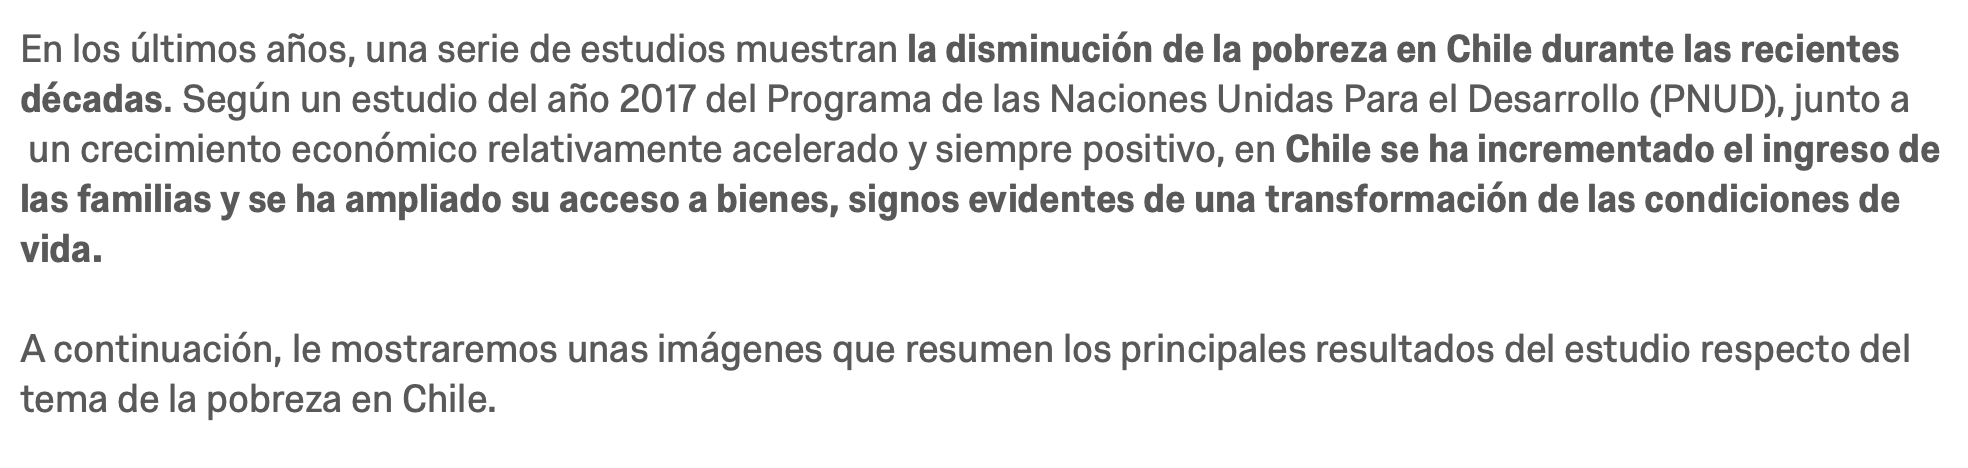
\includegraphics[height=6.0cm]{fig2.pdf}
\end{center}
\end{frame}


%Frame 19
\begin{frame}{} 
\begin{center}
	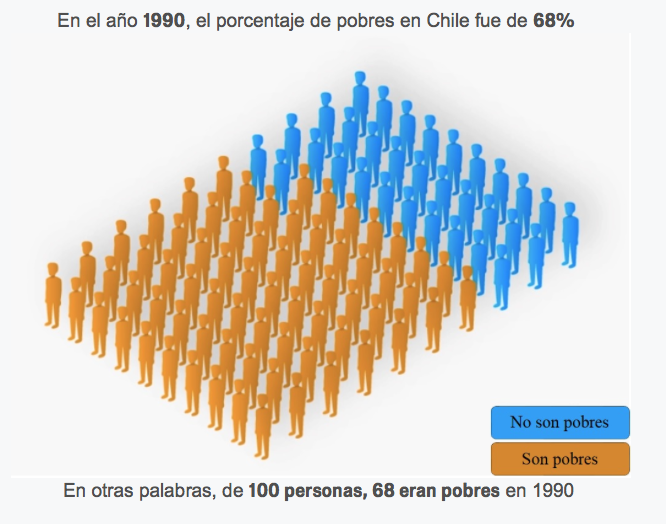
\includegraphics[height=7.0cm]{fig3.pdf}
\end{center}
\end{frame}

%Frame 19
\begin{frame}{} 
\begin{center}
	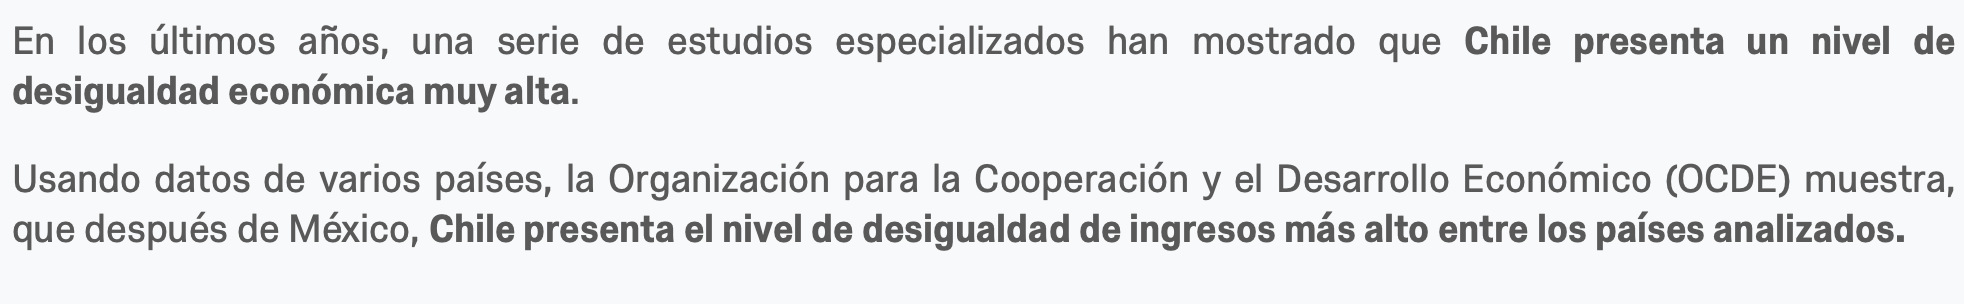
\includegraphics[height=4.0cm]{fig4.pdf}
\end{center}
\end{frame}

%Frame 19
\begin{frame}{} 
\begin{center}
	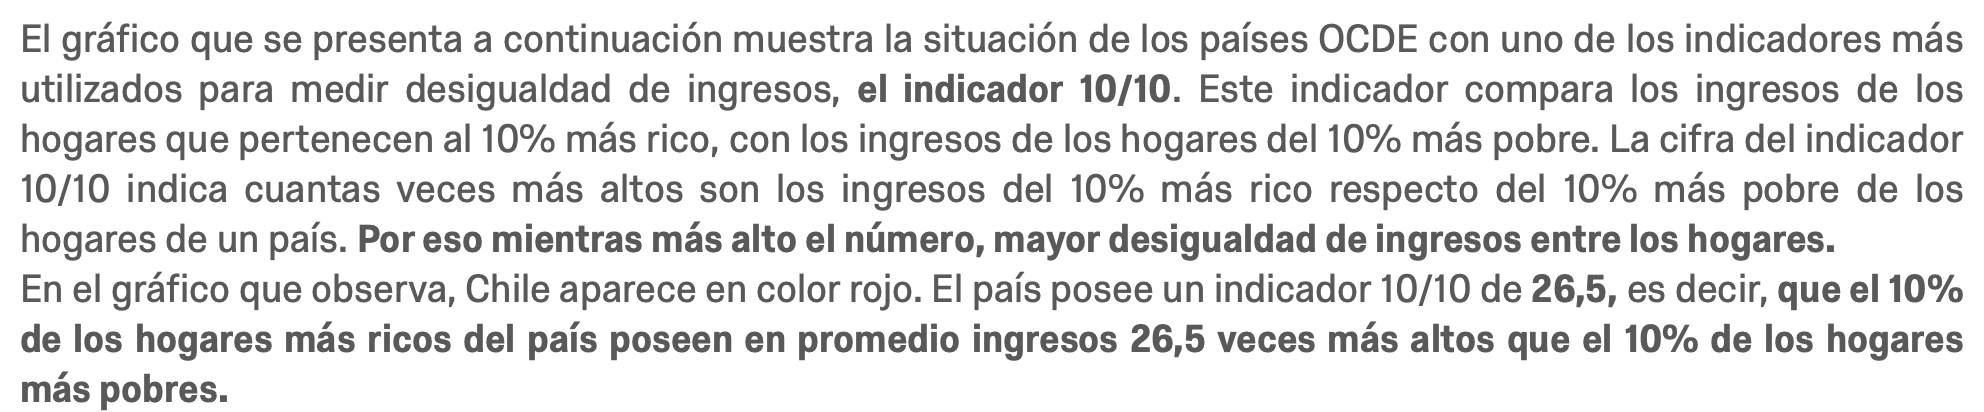
\includegraphics[height=5.9cm]{fig5.pdf}
\end{center}
\end{frame}

%Frame 19
\begin{frame}{} 
\begin{center}
	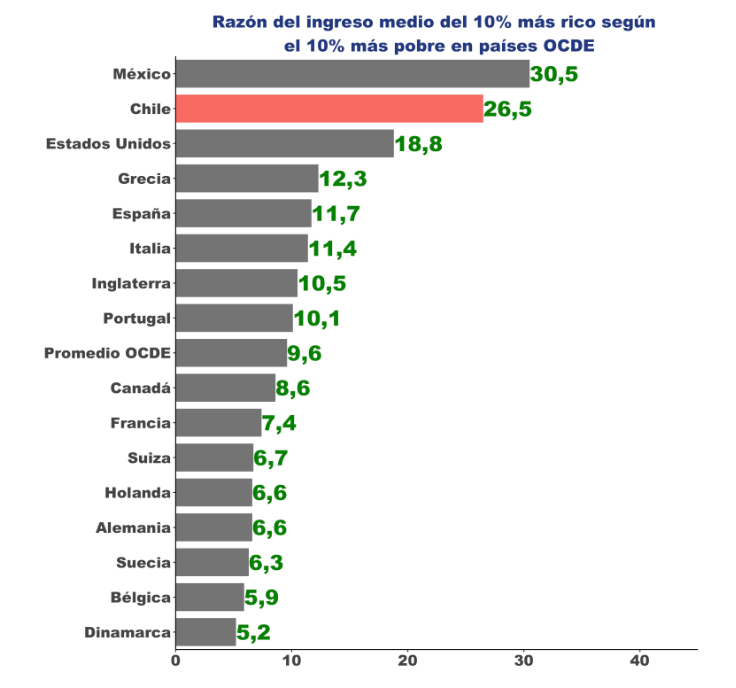
\includegraphics[height=7.0cm]{fig6.pdf}
\end{center}
\end{frame}

% slide
\begin{frame}{Outcomes}

\begin{itemize}
\justifying
\item  Opportunity beliefs: Battery of ISSP, social inequality module.
\medskip
	\begin{itemize}
	\justifying
	\item \textbf{Structural factors}: a) coming from a wealthy family and b) having well-educated parents.
	\medskip
	\item \textbf{Individual factors}: c) hard work and d) ambition.
	\medskip
	\item  {\color{red} Error}: we did not use item b) but e) having a good education yourself.
	\end{itemize}
\medskip
\item \textbf{Redistributive preferences}: willingness to pay higher taxes: i) to improve the level of health care for all people in Chile and ii) to reduce income differences between the rich and the poor in Chile.
\end{itemize}

\end{frame}

% slide
\begin{frame}{Covariates and method}

\begin{itemize}
\justifying
\item \textbf{Covariates}: socio-demographic characteristics and percepcion of pover-ty's evolution. All measures were applied before the treatments.
\medskip
\medskip
\item \textbf{Moderator}: Political knowledge (post-treatment).
\medskip
\medskip
\item \textbf{Methods}
	\begin{itemize}
	\justifying
	\item Average treatment effects (ATEs) with OLS regressions (HC2 standard errors).
	\item We control for covariates for efficiency. Covariates are balanced among treatment conditions.
	\item Multiple comparisons: Bonferroni correction.
	\end{itemize}
\end{itemize}
\end{frame}		


% Resultados
\section{Results}

\begin{frame} [allowframebreaks]
\frametitle{}

{\footnotesize

\begin{table}[H]
\caption{Effect of information about poverty and inequality on opportunity beliefs}
\begin{center}
\begin{tabular}{l D{)}{)}{11)2} D{)}{)}{11)2} D{)}{)}{11)2} }
\toprule
 & \multicolumn{1}{c}{Structural} & \multicolumn{1}{c}{Individual} & \multicolumn{1}{c}{Education} \\
\midrule
Condition: Poverty & 0.22 \; (0.17)      & 0.23 \; (0.10)^{*}   & 0.32 \; (0.11)^{**} \\
                   & [0.17]              & [0.28]               & [0.36]               \\
Condition: Inequality & 0.14 \; (0.18)      & 0.09 \; (0.11)       & 0.16 \; (0.12)      \\
                       & [0.11]              & [0.11]               & [0.18]               \\
\\
Controls       & Yes      & Yes       & Yes      \\
Observations       & 328                 & 328                  & 328  \\ 
R-squared         & 0.06                & 0.09                 & 0.07 \\
\bottomrule
\multicolumn{4}{l}{\scriptsize{$^{**}p<0.01$, $^*p<0.05$ (Two tailed test). Y-standardized coefficients in square brackets.}}
\end{tabular}
\label{table:coefficients}
\end{center}
\end{table}

} %End footnotesize


%Intro
\framebreak

{\footnotesize

\begin{table}[H]
\caption{Effect of information about poverty and inequality on opportunity beliefs}
\begin{center}
\begin{tabular}{l D{)}{)}{11)2} D{)}{)}{11)2} D{)}{)}{11)2} }
\toprule
 & \multicolumn{1}{c}{Structural} & \multicolumn{1}{c}{Individual} & \multicolumn{1}{c}{Education} \\
\midrule
Condition: Poverty & 0.22 \; (0.17)      & 0.23 \; (0.10)^{*}   & 0.32 \; (0.11)^{**} \\
                   & [0.17]              & [0.28]               & [0.36]               \\
Condition: Inequality & 0.14 \; (0.18)      & 0.09 \; (0.11)       & 0.16 \; (0.12)      \\
                       & [0.11]              & [0.11]               & [0.18]               \\
\\
Controls       & Yes      & Yes       & Yes      \\
Observations       & 328                 & 328                  & 328  \\ 
R-squared         & 0.06                & 0.09                 & 0.07 \\
\bottomrule
\multicolumn{4}{l}{\scriptsize{$^{**}p<0.01$, $^*p<0.05$ (Two tailed test). Y-standardized coefficients in square brackets.}}
\end{tabular}
\label{table:coefficients}
\end{center}
\end{table}

} %End footnotesize


\begin{itemize}
\justifying
\item We do not find significant effects on redistributive preferences but there is some evidence for political knowledge as moderator.
\end{itemize}

\end{frame}


% Discusión
\section{Discussion}

\begin{frame} [allowframebreaks]
\frametitle{}

\begin{itemize}
\justifying
\item Significant effect of poverty's information on \textit{having a good education yourself}. 
\medskip
\medskip
\medskip
\item Opportunity model of beliefs about economic inequality
\medskip
	\begin{enumerate}
	\justifying
	\item \textbf{Open question I}: Descriptive analysis suggests a rising demand for redistribution in a context of {\color{red}increasing economic opportunities}.
    \medskip
    \item \textbf{Open question II}: Explanatory mechanisms of the effect of perceptions of economic inequality on opportunity beliefs.
	\end{enumerate}
\end{itemize}

\end{frame}



%Discusión
\begin{frame}{Design of final study: two experiments}

\begin{enumerate}
\justifying
\item \textbf{Study 1: Effect of poverty's information on opportunity beliefs}
	\begin{itemize}
	\justifying
	\item Online Panel by using SSI with three waves: a) first to collect pre-treatment information; b) treatment; c) follow up to evaluate persistence of the effects.
	\medskip
	\item To include all relevant items to measure opportunity beliefs.
	\medskip
	\item Moderation (political knowledge): direction? 
	\end{itemize}
\medskip
\item \textbf{Study 2: Effects of poverty's information on support for specific social policies (gratuidad and pension reforms)}
	\begin{itemize}
	\justifying
	\item Online Panel by using SSI with three waves: a) first to collect pre-treatment information; b) treatment; c) follow up to evaluate persistence of the effects.
	\medskip
	\item Redistributive preferences vs. attitudes about specific policies.
	\medskip
	\item To evaluate mediation of opportunity beliefs.
	\medskip
	\end{itemize}
\medskip
\item Registration of pre-analysis plan.	
\end{enumerate}	



\end{frame}


\end{document}




























